\chapter{Resummation using Wilson Lines}\label{chap:Resummation in QCD}
In this chapter we will take a closer look at how we can deal with the large logarithms in the threshold region. First we will take a classical approach to eikonal exponentiation in an Abelian theory, following a similar line as Steven Weinberg \cite{Weinberg:1972rt}. The generalization to non-Abelian theories is not straightforward. This is of course due to the non-commutivity between non-Abelian gauge fields. The proof exist in the literature, and the result is known as the \emph{non-Abelian eikonal exponentiation theorem} \cite{Gatheral:1983cz,Frenkel:1984pz,Laenen:2008gt}. We will not cover this generalization as it would take us to far from our main purpose, but the above references can be sought out for more detail. 

After we have seen how amplitudes exponentiate, we will move on to discuss several factorization properties of cross sections in QCD. First, we will introduce the Mellin space formalism where we take a Mellin transform of the hadronic cross section and show how it factorizes. Then we go on and use factorization theorems to fully factorize the cross section in the threshold regime by using parton-in-parton distributions. After the cross section has been fully factorized into hard, soft and collinear parts we will use Wilson lines to construct an eikonal cross section that governs the soft radiation. Then we will briefly discuss the renormalization properties of Wilson lines and make an explicit calculation of the cusp anomalous dimension to one-loop order. 

With the introduction of the cusp anomalous dimension we discuss the renormalization group equation for parton-in-parton distributions and show that it is given in terms of the cusp anomalous dimension. The non-Abelian exponentiation theorem will then be used to find an exponentiated eikonal cross section. After we have found the exponentiated cross section we will take the discussion to the level of the hadronic cross section again. We will discuss possible ways of evaluating the inverse Mellin transform in order to obtain a cross section in real space. 


\section{Exponentiation}\label{sec:exponentiation}
In \cref{sec:Drell-Yan Hadronic Cross Section}, we dealt with a fixed order calculation for the Drell-Yan process. Due to soft gluon radiation from the hard quark lines, we identified large logarithmic contributions to the cross-section in the threshold region, i.e. $z\rightarrow 1$. As these large effects appear at all orders, they spoil the convergent behaviour of the series expansion in the strong coupling. To perform an all-order calculation in the full theory of QCD is an impossible task, but with certain approximations, these large contributions can be resummed.

Resummation of large logarithmic contributions was first demonstrated in \cite{1961AnPhy..13..379Y}, where the radiation of photons in QED was considered. The resummation was done by using the eikonal approximation, i.e. the photons are restricted to be soft. The crucial feature of the eikonal approximation is that scattering amplitudes exponentiate, with the consequence that one can compute the logarithm of the amplitude via a set of simplified rules. Therefore, we can access all order information from low-order perturbative calculations, which simplifies calculations substantially. Using this approximation, a scattering amplitude $\mathcal{M}$ describing multiple soft photon radiation can be written on the form
\begin{align}\label{eq:Soft Abelian amplitude}
    \mathcal{M}=\mathcal{M}_{0}\exp(\sum W_{c})\,,
\end{align}
where $\mathcal{M}_{0}$ is the amplitude without soft photon radiation, and the exponential has a sum over all connected Feynman diagrams $W_{c}$, involving soft photon emission only. Since QED is an Abelian gauge theory, the emitted photons will not interact and the amplitude factorizes, leading to an exponentiation of the amplitude. 

For a non-Abelian gauge theory, such as QCD, this simple factorization no longer applies as the gluons interact with each other. Nevertheless, in \cite{Sterman:1981jc}, it was observed that one could achieve exponentiation by using the eikonal approximation also in the case of QCD. The formal proof of this observation was later provided in \cite{Gatheral:1983cz, Frenkel:1984pz}, where the structure of the exponent is much more complicated due to the non-commutativity of the colour matrices. The non-abelian analogue of \cref{eq:Soft Abelian amplitude} can then be written on schematic form as
\begin{align}
    \mathcal{M}=\mathcal{M}_{0}\exp(\sum \Bar{c}_{W} W)\,,
\end{align}
where the soft gluons are emitted from two hard partons connected by a colour singlet vertex, which is exactly the case considered in the Drell-Yan process. The sum in the exponent involves Feynman diagrams $W$, called \emph{webs} in the literature, and $\Bar{c}_{W}$ are modified colour factors which in general differ from the usual colour factors $c_W$ using standard Feynman rules. We will encounter these webs later on, but we will not cover the details of their properties\footnote{This is an extensive topic, so for more detail about webs, see e.g. \cite{White:2015wha,Berger_2002,Laenen:2008gt,article}.}.

We will now show how the structure in \cref{eq:Soft Abelian amplitude} appears by considering the all order process of photon emission from a final state fermion-antifermion creation process. We will not do this by explicitly using Wilson lines, but we will again see that this it is equivalent.

%%%%%%%%%%%%%%%%%%%%%%%%%%%%%%%%%%%%%%%%%%%%%%%%
\subsection*{Eikonal Exponentiation in QED}\label{sec:Eikonal}
\begin{figure}
    \centering
    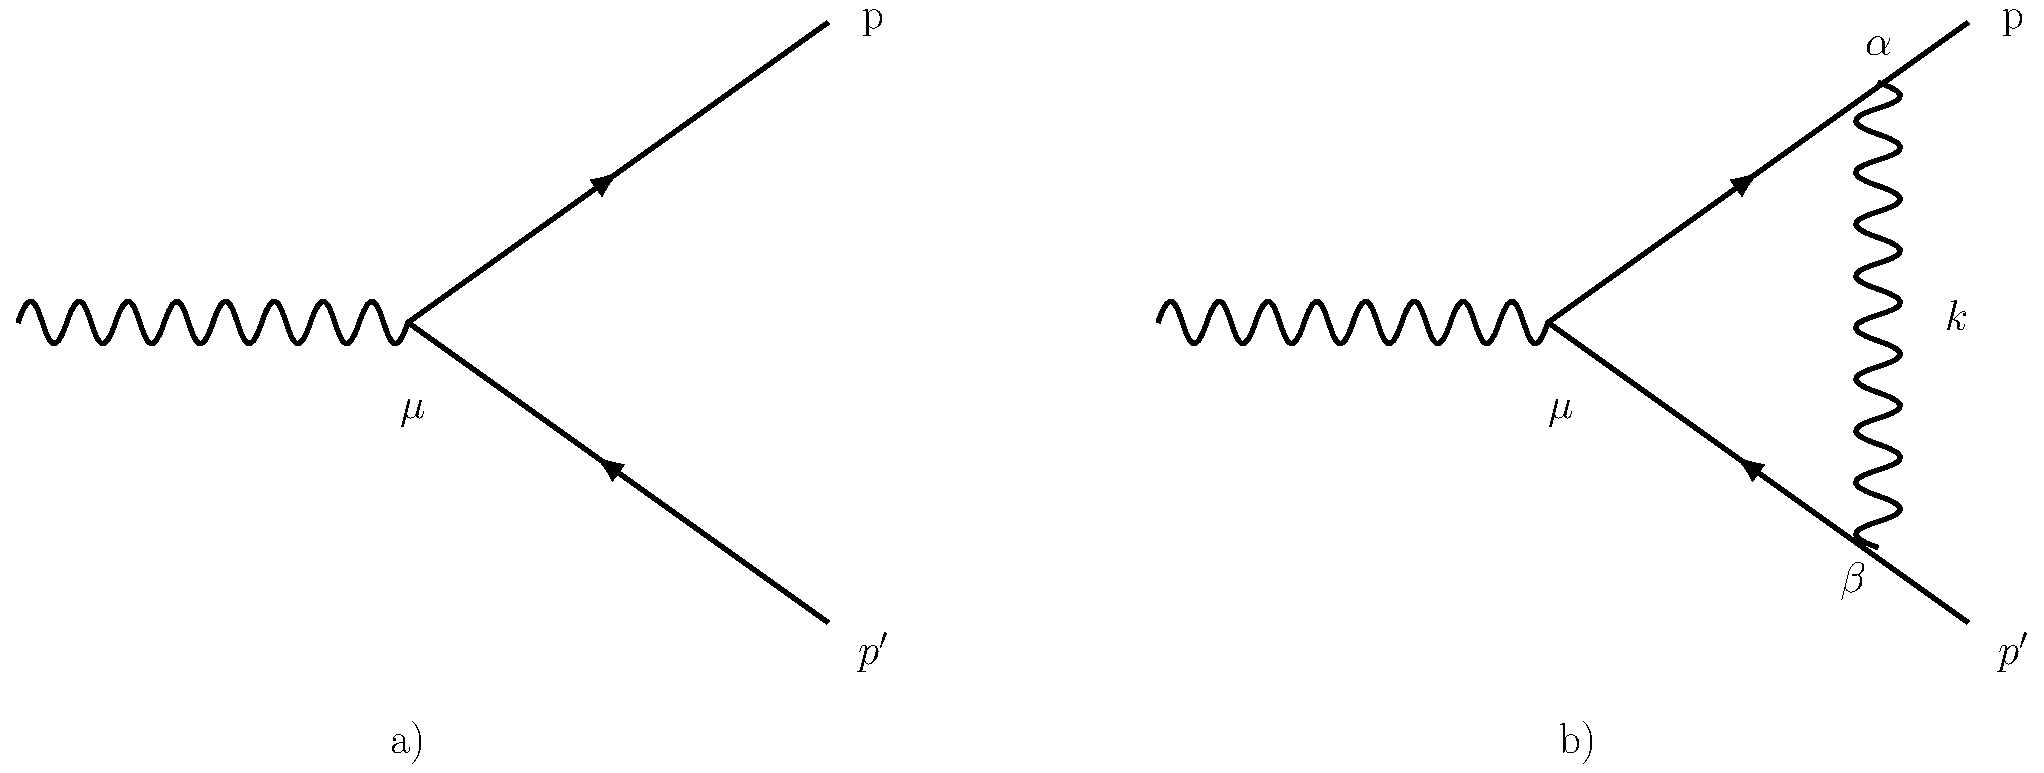
\includegraphics[scale=0.3]{Figures/photonvertexloop.pdf}
    \caption{Leading order and $\mathcal{O}(\alpha)$ correction to virtual photon decay.}
    \label{fig:photon diagrams}
\end{figure}
In this section we will look at the exponentiation of soft photon emission. 
Let us start by considering the amplitude of an off-shell photon decaying to a massless fermion-antifermion pair, see \cref{fig:photon diagrams}. The leading order amplitude is given by
\begin{align}
    \mathcal{M}_{0}=\Bar{u}(p)\gamma^{\mu}v(p')\,,
\end{align}
where coupling factors have been neglected for simplicity. If we now consider the correction, where a photon is emitted from the final state, we get the amplitude
\begin{align}
    \mathcal{M}_{1}=\int\frac{d^{d}k}{(2\pi)^{d}}\Bar{u}(p)\gamma^{\alpha}\frac{(\slashed{p}-\slashed{k})}{(p-k)^{2}}\gamma^{\mu}\frac{(\slashed{k}-\slashed{p'})}{(k-p')^{2}}\gamma^{\beta}v(p')D_{\alpha\beta}(k)\,,
\end{align}
where $D_{\alpha\beta}(k)$ is the photon propagator. 

As we showed in \cref{sec:wilson line properties} the eikonal approximation corresponds to taking the soft limit $k\rightarrow 0$, such that we can neglect $\slashed{k}$ in the numerator and $k^{2}$ in the denominator of the fermion propagators. If we also assume that the fermions are massless, $p^{2}=0$, we get the much simpler eikonal amplitude
\begin{align}\label{eq:factorized eikonal 1 photon amplitude}
    \mathcal{M}_{1}&=\int\frac{d^{d}k}{(2\pi)^{d}}\Bar{u}(p)\gamma^{\alpha}\Big(-\frac{\slashed{p}}{2p\cdot k}\Big)\gamma^{\mu}\Big(\frac{\slashed{p'}}{2p\cdot k}\Big)\gamma^{\beta}v(p')D_{\alpha\beta}(k)\nonumber
    \\
    &=\int\frac{d^{d}k}{(2\pi)^{d}}\big[\bar{u}(p)\gamma^{\mu}v(p'){\big]}\Big(-\frac{p^{\alpha}}{p\cdot k}\Big)\Big(\frac{p'^{\beta}}{p\cdot k}\Big)D_{\alpha\beta}(k)\nonumber
    \\
    &=\mathcal{M}_{0}\int\frac{d^{d}k}{(2\pi)^{d}}\Big(-\frac{p^{\alpha}}{p\cdot k}\Big)\Big(\frac{p'^{\beta}}{p\cdot k}\Big)D_{\alpha\beta}(k)\,,
\end{align}
where we in the second step used the Dirac algebra $\{\gamma^{\mu},\gamma^{\nu}\}=2g^{\mu\nu}$ and the massless Dirac equation, $\bar{u}(p)\slashed{p}=0$ and $\slashed{p'}v(p')=0$. We observe that the tree-level amplitude has been factored out, and contains no divergences. This result is actually an example of factorization of soft physics from hard physics, where the soft part is described by the integral and the hard part is the leading order amplitude $\mathcal{M}_{0}$. The physical reason for this factorization is that the momentum of the soft photon is to low to resolve the inner structure of the hard process. 

Another important observation is that we can define the terms inside the brackets as an eikonal Feynman rule\footnote{This is of course closely related to the Wilson line rules we derived in \cref{sec:wilson line properties}, with the distinction that this is an Abelian theory.}

\begin{fmffile}{ee}
\begin{align}
\begin{gathered}
\begin{fmfgraph*}(45,40)
\fmfleft{i}
\fmfright{o}
\fmf{plain}{i,v3}
\fmf{plain}{v3,o}
\fmffreeze   % freezing the drawn elements
\fmfright{v3,o3}   % adding two more vertices
\fmfforce{(0.5w,0.5h)}{v3}   % setting position of the first vertex
\fmfforce{(0.5w,0h)}{o3}   % setting position of the second vertex
\fmfdot{v3}   % drawing the first vertex with a dot
\fmf{photon, label=$k\downarrow$, l.side=left}{v3,o3}   % drawing a gluon line
\end{fmfgraph*}
\end{gathered}\hspace{0.6cm}&=\frac{p^{\mu}}{p\cdot k}\,.\hspace{2.36cm}\text{Eikonal vertex}\label{eq:Wilson vertex}
\end{align}
\end{fmffile}
This actually means that we can think of the factors multiplying the tree-level amplitude in \cref{eq:factorized eikonal 1 photon amplitude} as a new type of Feynman diagrams, which are \emph{subdiagrams} of the full amplitude. 
\begin{figure}
    \centering
    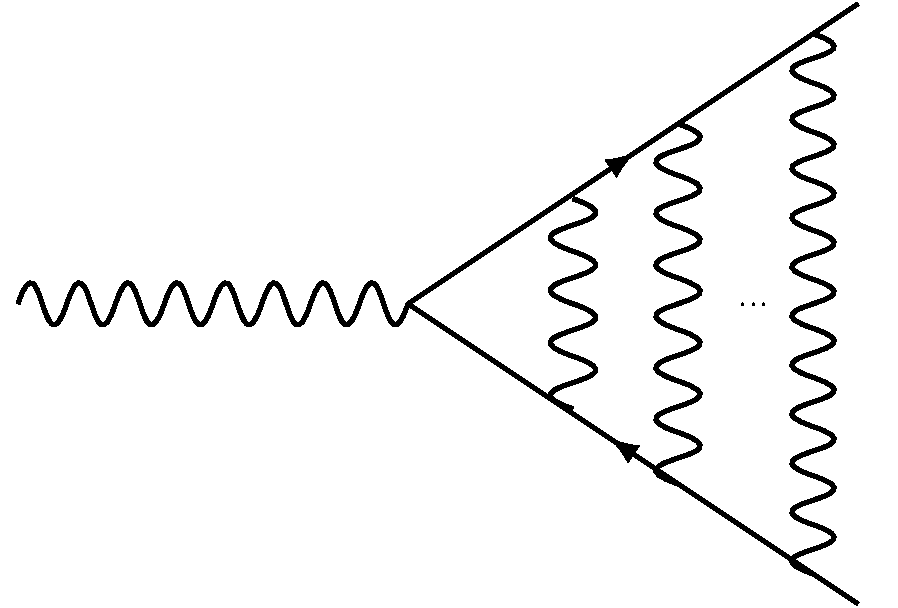
\includegraphics[scale=0.4]{Figures/LadderDiagram.pdf}
    \caption{Ladder diagram of $n$ soft photon emission.}
    \label{fig:Ladder diagram}
\end{figure}

The next step is to generalize to the emission of $n$ soft photons, so let us start with the diagram \cref{fig:Ladder diagram}, where none of the photon lines cross each other, called a \emph{ladder diagram}. This amplitude is given by
\begin{align}\label{eq:nth amplitude}
    \mathcal{M}^{(n)}=\Big(\prod_{i=1}^{n}\int\frac{d^{d}k_i}{(2\pi)^{d}}\Big)\bar{u}(p)\mathcal{E}^{\alpha_1\dots\alpha_n}(p,k_{i})\gamma^{\mu}\mathcal{E}^{\beta_1\dots\beta_n}(p',k_{i})v(p')D_{\alpha_1\beta_1}(k_1)\dots D_{\alpha_n\beta_n}(k_n)\,,
\end{align}
where we have collected the product of fermion propagators and the gamma matrices from the corresponding vertices into $\mathcal{E}$ in the following way
\begin{align}
    \mathcal{E}^{\alpha_1\dots\alpha_n}(p,k_{i})=\frac{\gamma^{\alpha_1}(\slashed{p}-\slashed{k_1})\cdots\gamma^{\alpha_n}(\slashed{p}-\slashed{k_1}- \dots -\slashed{k_n})}{(p-k_1)^{2}\cdots(p-k_1-\dots k_n)^{2}}\,,
\end{align}
and by taking the eikonal approximation this can be simplified to 
\begin{align}
    \mathcal{E}^{\alpha_1\dots\alpha_n}(p,k_{i})=\frac{\bar{u}(p)\gamma^{\alpha_1}\slashed{p}\gamma^{\alpha_2}\slashed{p}\cdots\gamma^{\alpha_n}\slashed{p}}{(-2p\cdot k_1)\cdots (-2p\cdot(k_1+\cdots+k_n)}\,,
\end{align}
which can be further simplified by permuting the gamma matrices using the Dirac algebra and use that $\bar{u}(p)\slashed{p}=0$, giving
\begin{align}
    \bar{u}(p)\mathcal{E}^{\alpha_1\dots\alpha_n}&=\frac{(-1)^{n}\bar{u}(p)p^{\alpha_1}\cdots p^{\alpha_n}}{p\cdot k_1\cdots p\cdot(k_1+\dots +k_n)}\,,
    \\
    \mathcal{E}^{\beta_1\dots\beta_n}v(p')&=\frac{p'^{\beta_1}\cdots p'^{\beta_n}\,v(p')}{p'\cdot k_1\cdots p'\cdot(k_1+\dots +k_n)}\,,
\end{align}
where the factors of $2$ cancels from those in the Dirac algebra, see \cref{eq:Dirac algebra}. 
Combining these two expressions into \cref{eq:nth amplitude}, we get
\begin{align}\label{eq:nth amplitude rewritten}
    \mathcal{M}^{(n)}=\mathcal{M}_{0}\Big(\prod_{i=1}^{n}\int\frac{d^{d}k_i}{(2\pi)^{d}}\Big)\Big[\frac{(-1)^{n}p^{\alpha_1}\cdots p^{\alpha_n}\,p'^{\beta_1}\cdots p'^{\beta_n}\,D_{\alpha_1\beta_1}(k_1)\cdots D_{\alpha_n\beta_n}(k_n)}{p\cdot k_1\cdots p\cdot(k_1+\dots +k_n)\,p'\cdot k_1\cdots p'\cdot(k_1+\dots +k_n)}\Big]\,.
\end{align}

This reveals an intricate dependency on the photon momenta $k_i$, as they are coupled along both the fermion and anti-fermion line. However, we have only considered the ladder diagram where the photons are emitted in the order $k_1\dots k_n$. Therefore, we must sum over all diagrams to this order, meaning we must sum over all permutations of the emitted photon momenta. We start by fixing the order of photon emission on the anti-fermion line, and sum over permutations on the fermion line. If we let $\pi$ denote a permutation of $(1,2,\dots,n)$, which maps to $(\pi_1,\pi_2,\dots \pi_n)$, the sum over diagrams correspond to making the following substitution
\begin{align*}
    \frac{1}{p\cdot k_1\cdots p\cdot(k_1+\dots +k_n)}\rightarrow \sum_{\pi}\frac{1}{p\cdot k_{\pi_1}\cdots p\cdot(k_{\pi_1}+\dots +k_{\pi_n})}\,.
\end{align*}
Then we can make use of the so-called \emph{eikonal identity}\footnote{This identity can be proven by using the Wilson lines we considered in \cref{sec:wilson line properties}, but for a standard derivation we refer the reader to \cite{Peskin:257493}.}
\begin{align}
    \sum_{\pi}\frac{1}{p\cdot k_{\pi_1}\cdots p\cdot(k_{\pi_1}+\dots +k_{\pi_n})}=\prod_{i=1}^{n}\frac{1}{p\cdot k_i}\,.
\end{align}
If this seems mysterious, let us show a simple example that highlights how this works. For the simple case of $n=2$, we have that
\begin{align}
    \frac{1}{p\cdot k_1\,p\cdot(k_1+k_2)}+\frac{1}{p\cdot k_2\,p\cdot(k_1+k_2)}=\frac{1}{p\cdot k_1\,p\cdot k_2}\,,
\end{align}
which shows the structure.

So by using the eikonal identity we substantially simplify the dependence on the photon momenta for the fermion line, as they have decoupled from each other. We could hope to do the same on the anti-fermion line, but that is not possible as they have already been fixed. However, we can exploit that $k_i$ are dummy variables inside the integral. The integrand has a symmetric Lorentz structure under the permutation of any two momenta, which means that we can make the replacement
\begin{align}
    \Big(&\prod_{i=1}^{n}\int\frac{d^{d}k_i}{(2\pi)^{d}}\Big)\frac{1}{p'\cdot k_1\cdots p'\cdot(k_1+\dots +k_n)}\nonumber
    \\
    &=\frac{1}{n!}\Big(\prod_{i=1}^{n}\int\frac{d^{d}k_i}{(2\pi)^{d}}\Big)\sum_{\pi}\frac{1}{p'\cdot k_{\pi_1}\cdots p'\cdot(k_{\pi_1}+\dots +k_{\pi_n})}\nonumber
    \\
    &=\frac{1}{n!}\prod_{i=1}^{n}\int\frac{d^{d}k_i}{(2\pi)^{d}}\frac{1}{p'\cdot k_i}\,,
\end{align}
where we have used that there are $n!$ such permutations. 

Substituting these simplifications into \cref{eq:nth amplitude rewritten}, we get
\begin{align}
    \mathcal{M}^{(n)}&=\mathcal{M}_{0}\frac{1}{n!}\prod_{i=1}^{n}\int\frac{d^{d}k_i}{(2\pi)^{d}}\big(\frac{p^{\alpha_i}}{p\cdot k_i}\big)\big(\frac{-p'^{\beta_i}}{p'\cdot k_i}\big)D_{\alpha_i\beta_i}(k_i)\nonumber
    \\
    &=\mathcal{M}_{0}\frac{1}{n!}\Big[\int\frac{d^{d}k}{(2\pi)^{d}}\big(\frac{p^{\alpha}}{p\cdot k}\big)\big(\frac{-p'^{\beta}}{p'\cdot k}\big)D_{\alpha\beta}(k)\Big]^{n}\,.
\end{align}
This looks very much like the $n$th term in a Taylor expansion of an exponential. By using the eikonal approximation we have found the remarkable result that the sum over all $n$ photon graphs is given by the one-loop graph to the $n$th power! If we take the sum over all diagrams for any number of single soft photon emission, we find the all order amplitude
\begin{align}\label{eq:exponentiated amplitude}
    \mathcal{M}&=\sum_{n=1}^{\infty}\mathcal{M}^{(n)}=\mathcal{M}_{0}\exp\Big(\int\frac{d^{d}k}{(2\pi)^{d}}\big(\frac{p^{\alpha}}{p\cdot k}\big)\big(\frac{-p'^{\beta}}{p'\cdot k}\big)D_{\alpha\beta}(k)\Big)\,,
\end{align}
which demonstrates that the hard part factorizes from the soft part also in the all order case, with the addition that the soft part exponentiates. From the structure of \cref{eq:exponentiated amplitude}, we can write the amplitude on the factorized form
\begin{align}
    \mathcal{M}=\mathcal{H}\mathcal{S}\,,
\end{align}
where $\mathcal{H}$ is a hard scattering function and $\mathcal{S}$ is a soft scattering function. The hard function is finite, while the soft function contains all the soft and collinear divergences. It is important to note that we have only considered single photon emissions, but to be general one should in fact consider the case where the emitted photons could connect off the external lines, via fermion loops. This would extend the result in \cref{eq:exponentiated amplitude} to include the sum over all connected diagrams including loops in the exponent, see \cite{1961AnPhy..13..379Y}. 

As already mentioned the complexity increases substantially for a non-abelian gauge theory, and while the result has existed in literature for a long time \cite{Gatheral:1983cz,Frenkel:1984pz}, the proof is restricted to involve only two coloured external particles. This proof covers Drell-Yan like processes, but if the final state contains coloured particles as well this proof does not hold. This scenario has been studied in great detail and recent work has been done to improve it to include several coloured particles \cite{White:2015wha,Laenen:2008gt}. The proof is too advanced to go into detail on here, but the main idea is to use a path integral approach with Wilson lines as a source for creating particles from the vacuum. From there one uses the so-called replica method from statistical mechanics to show that the theory can be written as $N$ replicas leading to the structure of webs.


